% Options for packages loaded elsewhere
% Options for packages loaded elsewhere
\PassOptionsToPackage{unicode}{hyperref}
\PassOptionsToPackage{hyphens}{url}
\PassOptionsToPackage{dvipsnames,svgnames,x11names}{xcolor}
%
\documentclass[
  letterpaper,
  DIV=11,
  numbers=noendperiod]{scrartcl}
\usepackage{xcolor}
\usepackage{amsmath,amssymb}
\setcounter{secnumdepth}{-\maxdimen} % remove section numbering
\usepackage{iftex}
\ifPDFTeX
  \usepackage[T1]{fontenc}
  \usepackage[utf8]{inputenc}
  \usepackage{textcomp} % provide euro and other symbols
\else % if luatex or xetex
  \usepackage{unicode-math} % this also loads fontspec
  \defaultfontfeatures{Scale=MatchLowercase}
  \defaultfontfeatures[\rmfamily]{Ligatures=TeX,Scale=1}
\fi
\usepackage{lmodern}
\ifPDFTeX\else
  % xetex/luatex font selection
\fi
% Use upquote if available, for straight quotes in verbatim environments
\IfFileExists{upquote.sty}{\usepackage{upquote}}{}
\IfFileExists{microtype.sty}{% use microtype if available
  \usepackage[]{microtype}
  \UseMicrotypeSet[protrusion]{basicmath} % disable protrusion for tt fonts
}{}
\makeatletter
\@ifundefined{KOMAClassName}{% if non-KOMA class
  \IfFileExists{parskip.sty}{%
    \usepackage{parskip}
  }{% else
    \setlength{\parindent}{0pt}
    \setlength{\parskip}{6pt plus 2pt minus 1pt}}
}{% if KOMA class
  \KOMAoptions{parskip=half}}
\makeatother
% Make \paragraph and \subparagraph free-standing
\makeatletter
\ifx\paragraph\undefined\else
  \let\oldparagraph\paragraph
  \renewcommand{\paragraph}{
    \@ifstar
      \xxxParagraphStar
      \xxxParagraphNoStar
  }
  \newcommand{\xxxParagraphStar}[1]{\oldparagraph*{#1}\mbox{}}
  \newcommand{\xxxParagraphNoStar}[1]{\oldparagraph{#1}\mbox{}}
\fi
\ifx\subparagraph\undefined\else
  \let\oldsubparagraph\subparagraph
  \renewcommand{\subparagraph}{
    \@ifstar
      \xxxSubParagraphStar
      \xxxSubParagraphNoStar
  }
  \newcommand{\xxxSubParagraphStar}[1]{\oldsubparagraph*{#1}\mbox{}}
  \newcommand{\xxxSubParagraphNoStar}[1]{\oldsubparagraph{#1}\mbox{}}
\fi
\makeatother


\usepackage{longtable,booktabs,array}
\usepackage{calc} % for calculating minipage widths
% Correct order of tables after \paragraph or \subparagraph
\usepackage{etoolbox}
\makeatletter
\patchcmd\longtable{\par}{\if@noskipsec\mbox{}\fi\par}{}{}
\makeatother
% Allow footnotes in longtable head/foot
\IfFileExists{footnotehyper.sty}{\usepackage{footnotehyper}}{\usepackage{footnote}}
\makesavenoteenv{longtable}
\usepackage{graphicx}
\makeatletter
\newsavebox\pandoc@box
\newcommand*\pandocbounded[1]{% scales image to fit in text height/width
  \sbox\pandoc@box{#1}%
  \Gscale@div\@tempa{\textheight}{\dimexpr\ht\pandoc@box+\dp\pandoc@box\relax}%
  \Gscale@div\@tempb{\linewidth}{\wd\pandoc@box}%
  \ifdim\@tempb\p@<\@tempa\p@\let\@tempa\@tempb\fi% select the smaller of both
  \ifdim\@tempa\p@<\p@\scalebox{\@tempa}{\usebox\pandoc@box}%
  \else\usebox{\pandoc@box}%
  \fi%
}
% Set default figure placement to htbp
\def\fps@figure{htbp}
\makeatother





\setlength{\emergencystretch}{3em} % prevent overfull lines

\providecommand{\tightlist}{%
  \setlength{\itemsep}{0pt}\setlength{\parskip}{0pt}}



 


\KOMAoption{captions}{tableheading}
\makeatletter
\@ifpackageloaded{caption}{}{\usepackage{caption}}
\AtBeginDocument{%
\ifdefined\contentsname
  \renewcommand*\contentsname{Table of contents}
\else
  \newcommand\contentsname{Table of contents}
\fi
\ifdefined\listfigurename
  \renewcommand*\listfigurename{List of Figures}
\else
  \newcommand\listfigurename{List of Figures}
\fi
\ifdefined\listtablename
  \renewcommand*\listtablename{List of Tables}
\else
  \newcommand\listtablename{List of Tables}
\fi
\ifdefined\figurename
  \renewcommand*\figurename{Figure}
\else
  \newcommand\figurename{Figure}
\fi
\ifdefined\tablename
  \renewcommand*\tablename{Table}
\else
  \newcommand\tablename{Table}
\fi
}
\@ifpackageloaded{float}{}{\usepackage{float}}
\floatstyle{ruled}
\@ifundefined{c@chapter}{\newfloat{codelisting}{h}{lop}}{\newfloat{codelisting}{h}{lop}[chapter]}
\floatname{codelisting}{Listing}
\newcommand*\listoflistings{\listof{codelisting}{List of Listings}}
\makeatother
\makeatletter
\makeatother
\makeatletter
\@ifpackageloaded{caption}{}{\usepackage{caption}}
\@ifpackageloaded{subcaption}{}{\usepackage{subcaption}}
\makeatother
\usepackage{bookmark}
\IfFileExists{xurl.sty}{\usepackage{xurl}}{} % add URL line breaks if available
\urlstyle{same}
\hypersetup{
  pdftitle={Fundamentos de Deep Learning \& Neurônio Artificial},
  pdfauthor={Faculdade Infnet},
  colorlinks=true,
  linkcolor={blue},
  filecolor={Maroon},
  citecolor={Blue},
  urlcolor={Blue},
  pdfcreator={LaTeX via pandoc}}


\title{Fundamentos de Deep Learning \& Neurônio Artificial}
\usepackage{etoolbox}
\makeatletter
\providecommand{\subtitle}[1]{% add subtitle to \maketitle
  \apptocmd{\@title}{\par {\large #1 \par}}{}{}
}
\makeatother
\subtitle{Aula 01: O Perceptron, Ativações e o Caso da Creatina}
\author{Faculdade Infnet}
\date{2026-07-27}
\begin{document}
\maketitle


\subsection{Introdução ao Deep
Learning}\label{introduuxe7uxe3o-ao-deep-learning}

\begin{center}
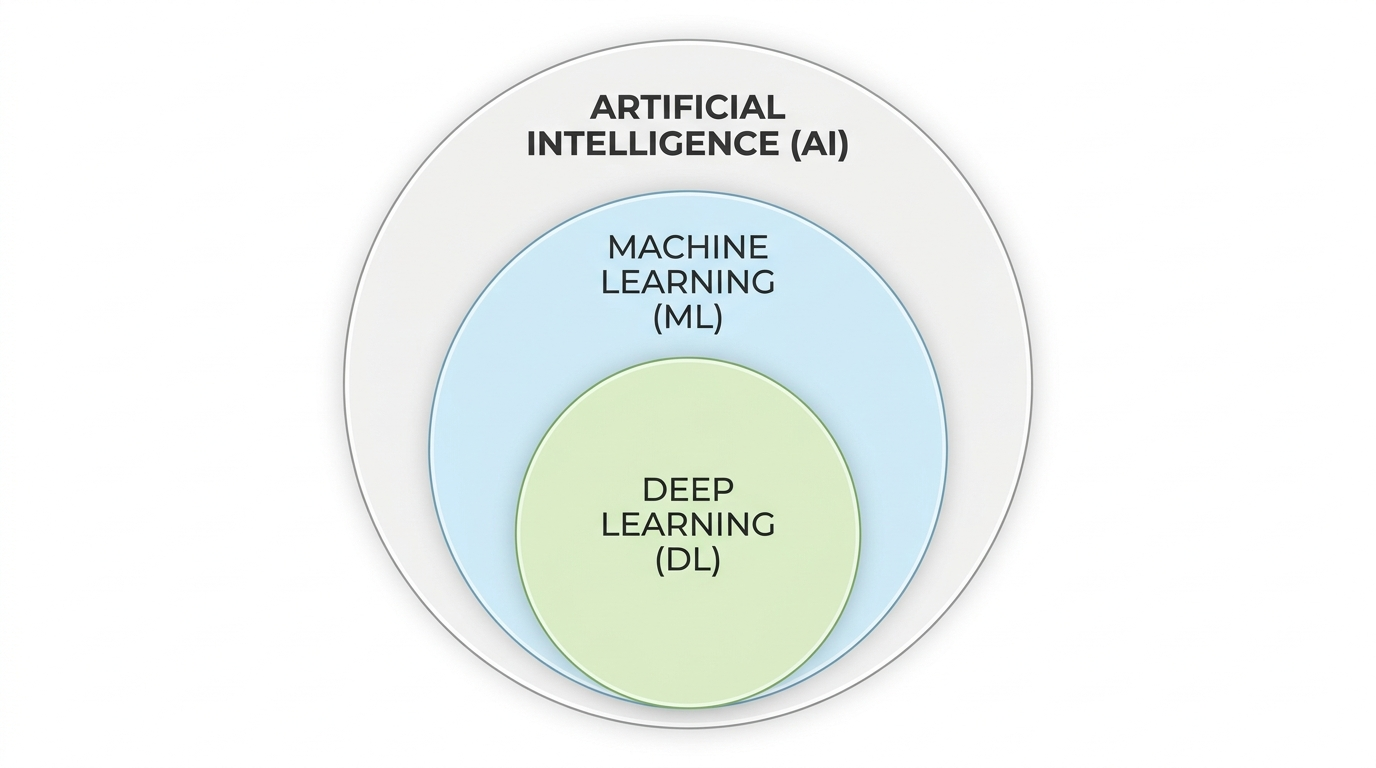
\includegraphics[width=0.65\linewidth,height=\textheight,keepaspectratio]{imagens/diagrama_venn.jpg}
\end{center}

\textbf{Falas do Apresentador:} ``Olá a todos! Sejam muito bem-vindos à
nossa primeira aula sobre Redes Neurais Profundas com PyTorch. Vejam a
imagem na tela. Ela representa graficamente a relação de inclusão entre
as três áreas mais faladas hoje. 1. \textbf{Inteligência Artificial
(IA)}: É a área mais ampla e de fora do diagrama, focada em sistemas que
simulam algum aspecto da inteligência humana. 2. \textbf{Machine
Learning (ML)}: É a subárea azul. Em vez de programar regras estritas na
mão, criamos algoritmos que aprendem regras e padrões de forma
estatística a partir de dados estruturados. 3. \textbf{Deep Learning
(DL)}: Representado na área verde interna. É um subcampo do ML focado em
processar dados altamente complexos (como imagens, áudio e texto)
utilizando arquiteturas com múltiplas camadas de neurônios artificiais.
Hoje, vamos focar no bloco elementar que está na base de todo o Deep
Learning: o Perceptron!''

\begin{center}\rule{0.5\linewidth}{0.5pt}\end{center}

\subsection{O Perceptron Clássico
(Genérico)}\label{o-perceptron-cluxe1ssico-genuxe9rico}

\begin{center}
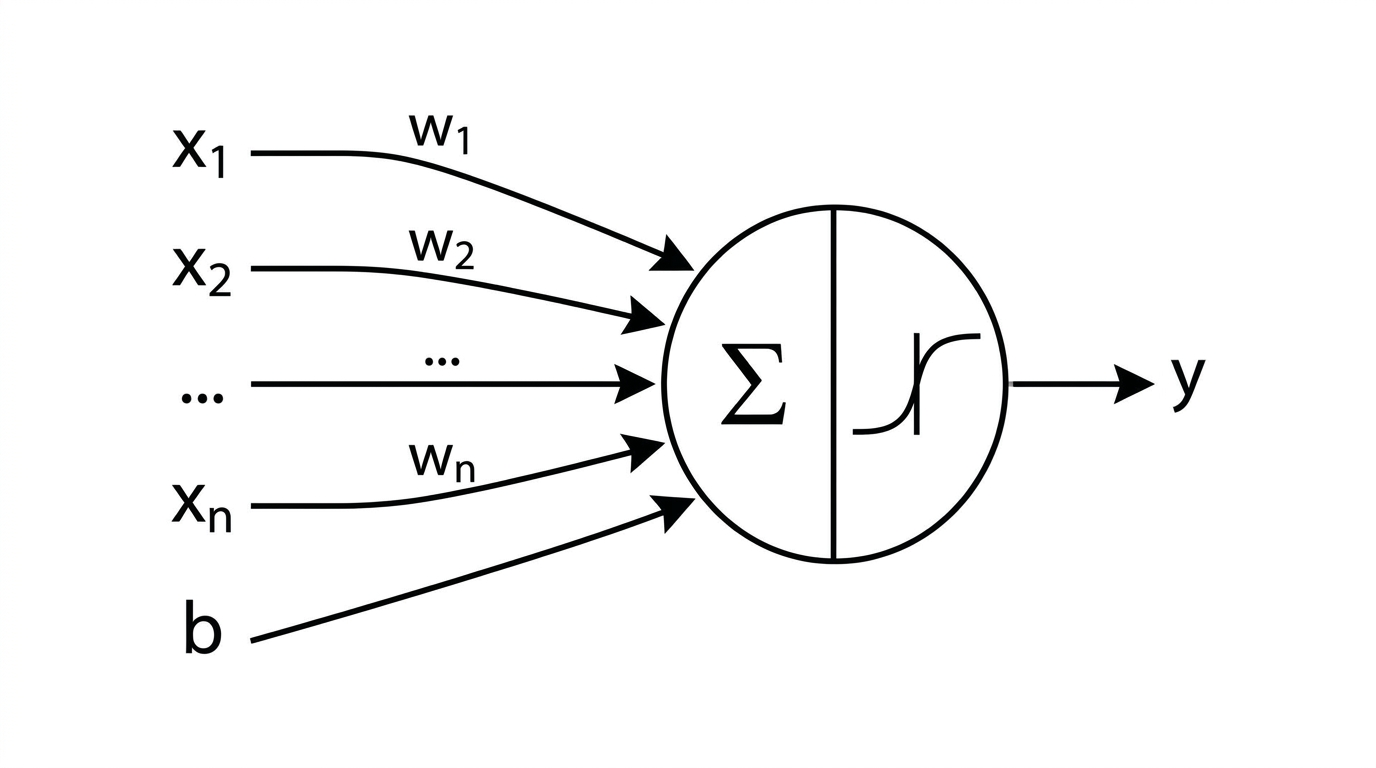
\includegraphics[width=0.7\linewidth,height=\textheight,keepaspectratio]{imagens/perceptron_generico.jpg}
\end{center}

\textbf{Falas do Apresentador:} ``Este é o modelo convencional e
clássico do Perceptron que vocês encontrarão na literatura e livros
acadêmicos. Ele é o processador básico de dados. Ele funciona recebendo
sinais de entrada genéricos (x1, x2, até x\_n). Cada entrada tem um peso
associado (w1, w2, até w\_n) que regula a força ou a importância desse
sinal. Temos também a entrada especial de Bias (viés, b). No núcleo do
neurônio, o processamento ocorre em duas etapas: Primeiro, calculamos
uma combinação linear, ou soma ponderada (z), multiplicando as entradas
pelos pesos e adicionando o viés. Segundo, passamos o valor resultante
por uma função de ativação `f(z)' para decidir o nível de disparo ou a
predição final `y'.''

\begin{center}\rule{0.5\linewidth}{0.5pt}\end{center}

\subsection{O Neurônio Artificial
(Aplicado)}\label{o-neuruxf4nio-artificial-aplicado}

\begin{center}
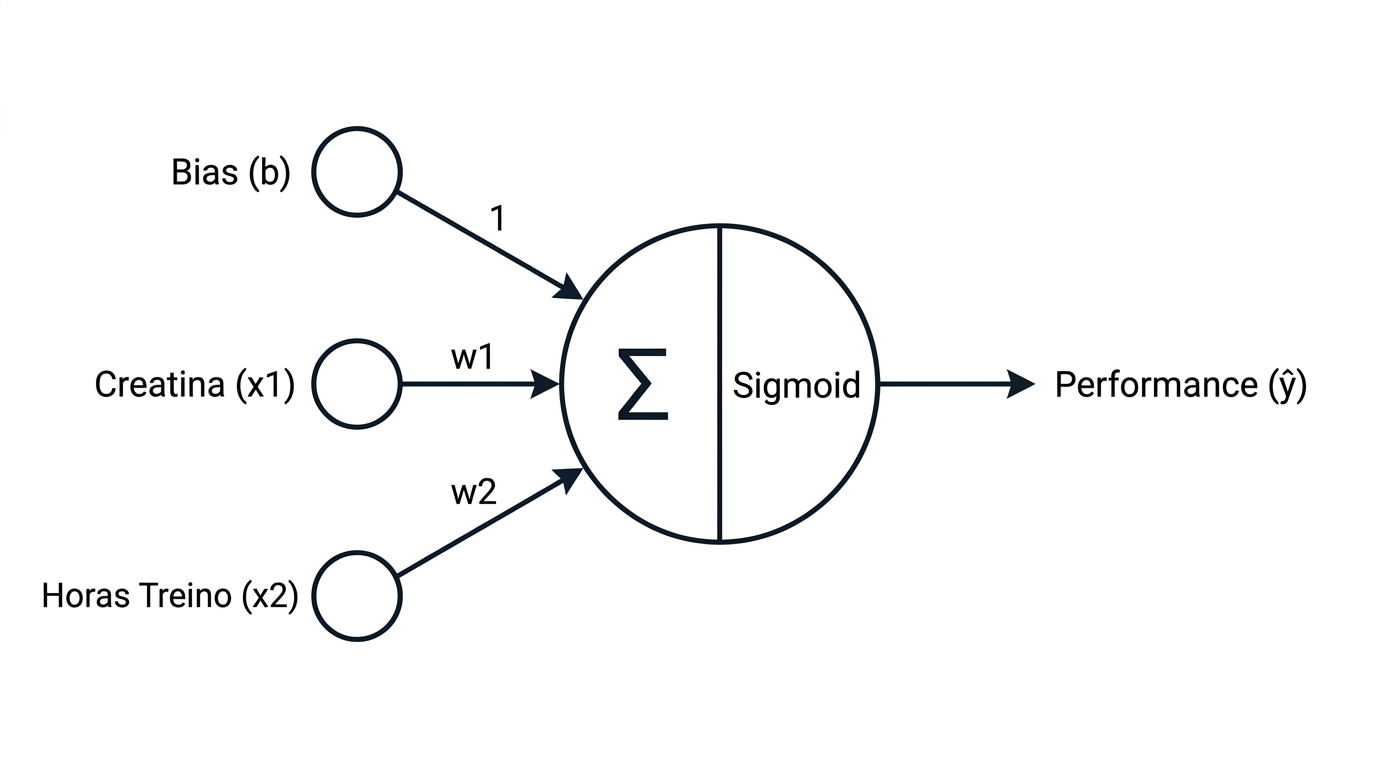
\includegraphics[width=0.7\linewidth,height=\textheight,keepaspectratio]{imagens/perceptron_aplicado.jpg}
\end{center}

\textbf{Falas do Apresentador:} ``Agora, observem a transição lógica do
modelo puramente abstrato para o nosso problema real de classificação
esportiva. As entradas genéricas `x' agora têm nomes palpáveis:
`Creatina (x1)' (dosagem diária em gramas) e `Horas de Treino (x2)'. Os
pesos (w1 e w2) vão definir o impacto de cada um desses hábitos no
rendimento do atleta. Nossa função de ativação abstrata é substituída
pela função matemática Sigmoid. A nossa saída predita é y-chapéu (ŷ),
indicando a probabilidade de o atleta atingir alta performance baseado
nestes hábitos.''

\begin{center}\rule{0.5\linewidth}{0.5pt}\end{center}

\subsection{A Matemática da
Decisão}\label{a-matemuxe1tica-da-decisuxe3o}

\[z = w_1 x_1 + w_2 x_2 + b\]

\textbf{Falas do Apresentador:} ``Neste slide, destacamos a equação da
Combinação Linear que ocorre dentro do neurônio: z = w1\emph{x1 + w2}x2
+ b. - \textbf{z}: É o potencial de decisão linear do modelo. -
\textbf{Entradas (x1, x2)}: Representam o consumo de Creatina em gramas
(x1) e as Horas de Treino semanais (x2). - \textbf{Pesos (w1, w2)}:
Regulam o impacto e a inclinação da fronteira de decisão no gráfico. -
\textbf{Viés (b)}: É o deslocamento da linha. Sem o viés b, a reta seria
forçada a passar pela origem (0,0), o que nos impediria de separar os
dados se a fronteira estivesse distante da origem. - Se z \textgreater{}
0, o potencial linear favorece a classe positiva (Alta Performance). Se
z \textless{} 0, favorece a classe regular.''

\begin{center}\rule{0.5\linewidth}{0.5pt}\end{center}

\subsection{A Função de Ativação
Sigmoid}\label{a-funuxe7uxe3o-de-ativauxe7uxe3o-sigmoid}

\[\hat{y} = \sigma(z) = \frac{1}{1 + e^{-z}}\]

\textbf{Falas do Apresentador:} ``O cálculo linear anterior gera valores
`z' que variam de menos infinito a mais infinito. Mas para dizer se um
atleta é 1 ou 0, precisamos de uma probabilidade entre 0 e 1. É aí que
entra a função Sigmoid, dada por 1 / (1 + e\^{}-z): - A Sigmoid achata
qualquer soma ponderada z para o intervalo {[}0, 1{]}. - Interpretamos
y-chapéu (ŷ) como a probabilidade de o atleta ser de Alta Performance. -
\textbf{Regra de Decisão}: Se ŷ \textgreater= 0.5 (50\%), classificamos
como Alta Performance (1). Se ŷ \textless{} 0.5, classificamos como
Performance Regular (0). - A fronteira de decisão exata ocorre em z = 0,
pois sigma(0) = 0.5.''

\begin{center}\rule{0.5\linewidth}{0.5pt}\end{center}

\subsection{Por que precisamos de
Ativações?}\label{por-que-precisamos-de-ativauxe7uxf5es}

\[y = W_2 (W_1 x + b_1) + b_2 = (W_2 W_1) x + (W_2 b_1 + b_2) = W_{eq} x + b_{eq}\]

\textbf{Falas do Apresentador:} ``Por que precisamos dessas funções nas
redes neurais? Se não usássemos nenhuma função de ativação, multiplicar
uma matriz de pesos por outra matriz de pesos resultaria em apenas uma
grande multiplicação linear. Como vemos na fórmula na tela, uma rede de
100 camadas sem ativação teria exatamente a mesma capacidade de
representação de um único neurônio linear! As funções de ativação
quebram essa linearidade. Elas atuam como dobradiças ou filtros
não-lineares nas transformações.''

\begin{center}\rule{0.5\linewidth}{0.5pt}\end{center}

\subsection{Visão Geral das Funções de
Ativação}\label{visuxe3o-geral-das-funuxe7uxf5es-de-ativauxe7uxe3o}

\begin{center}
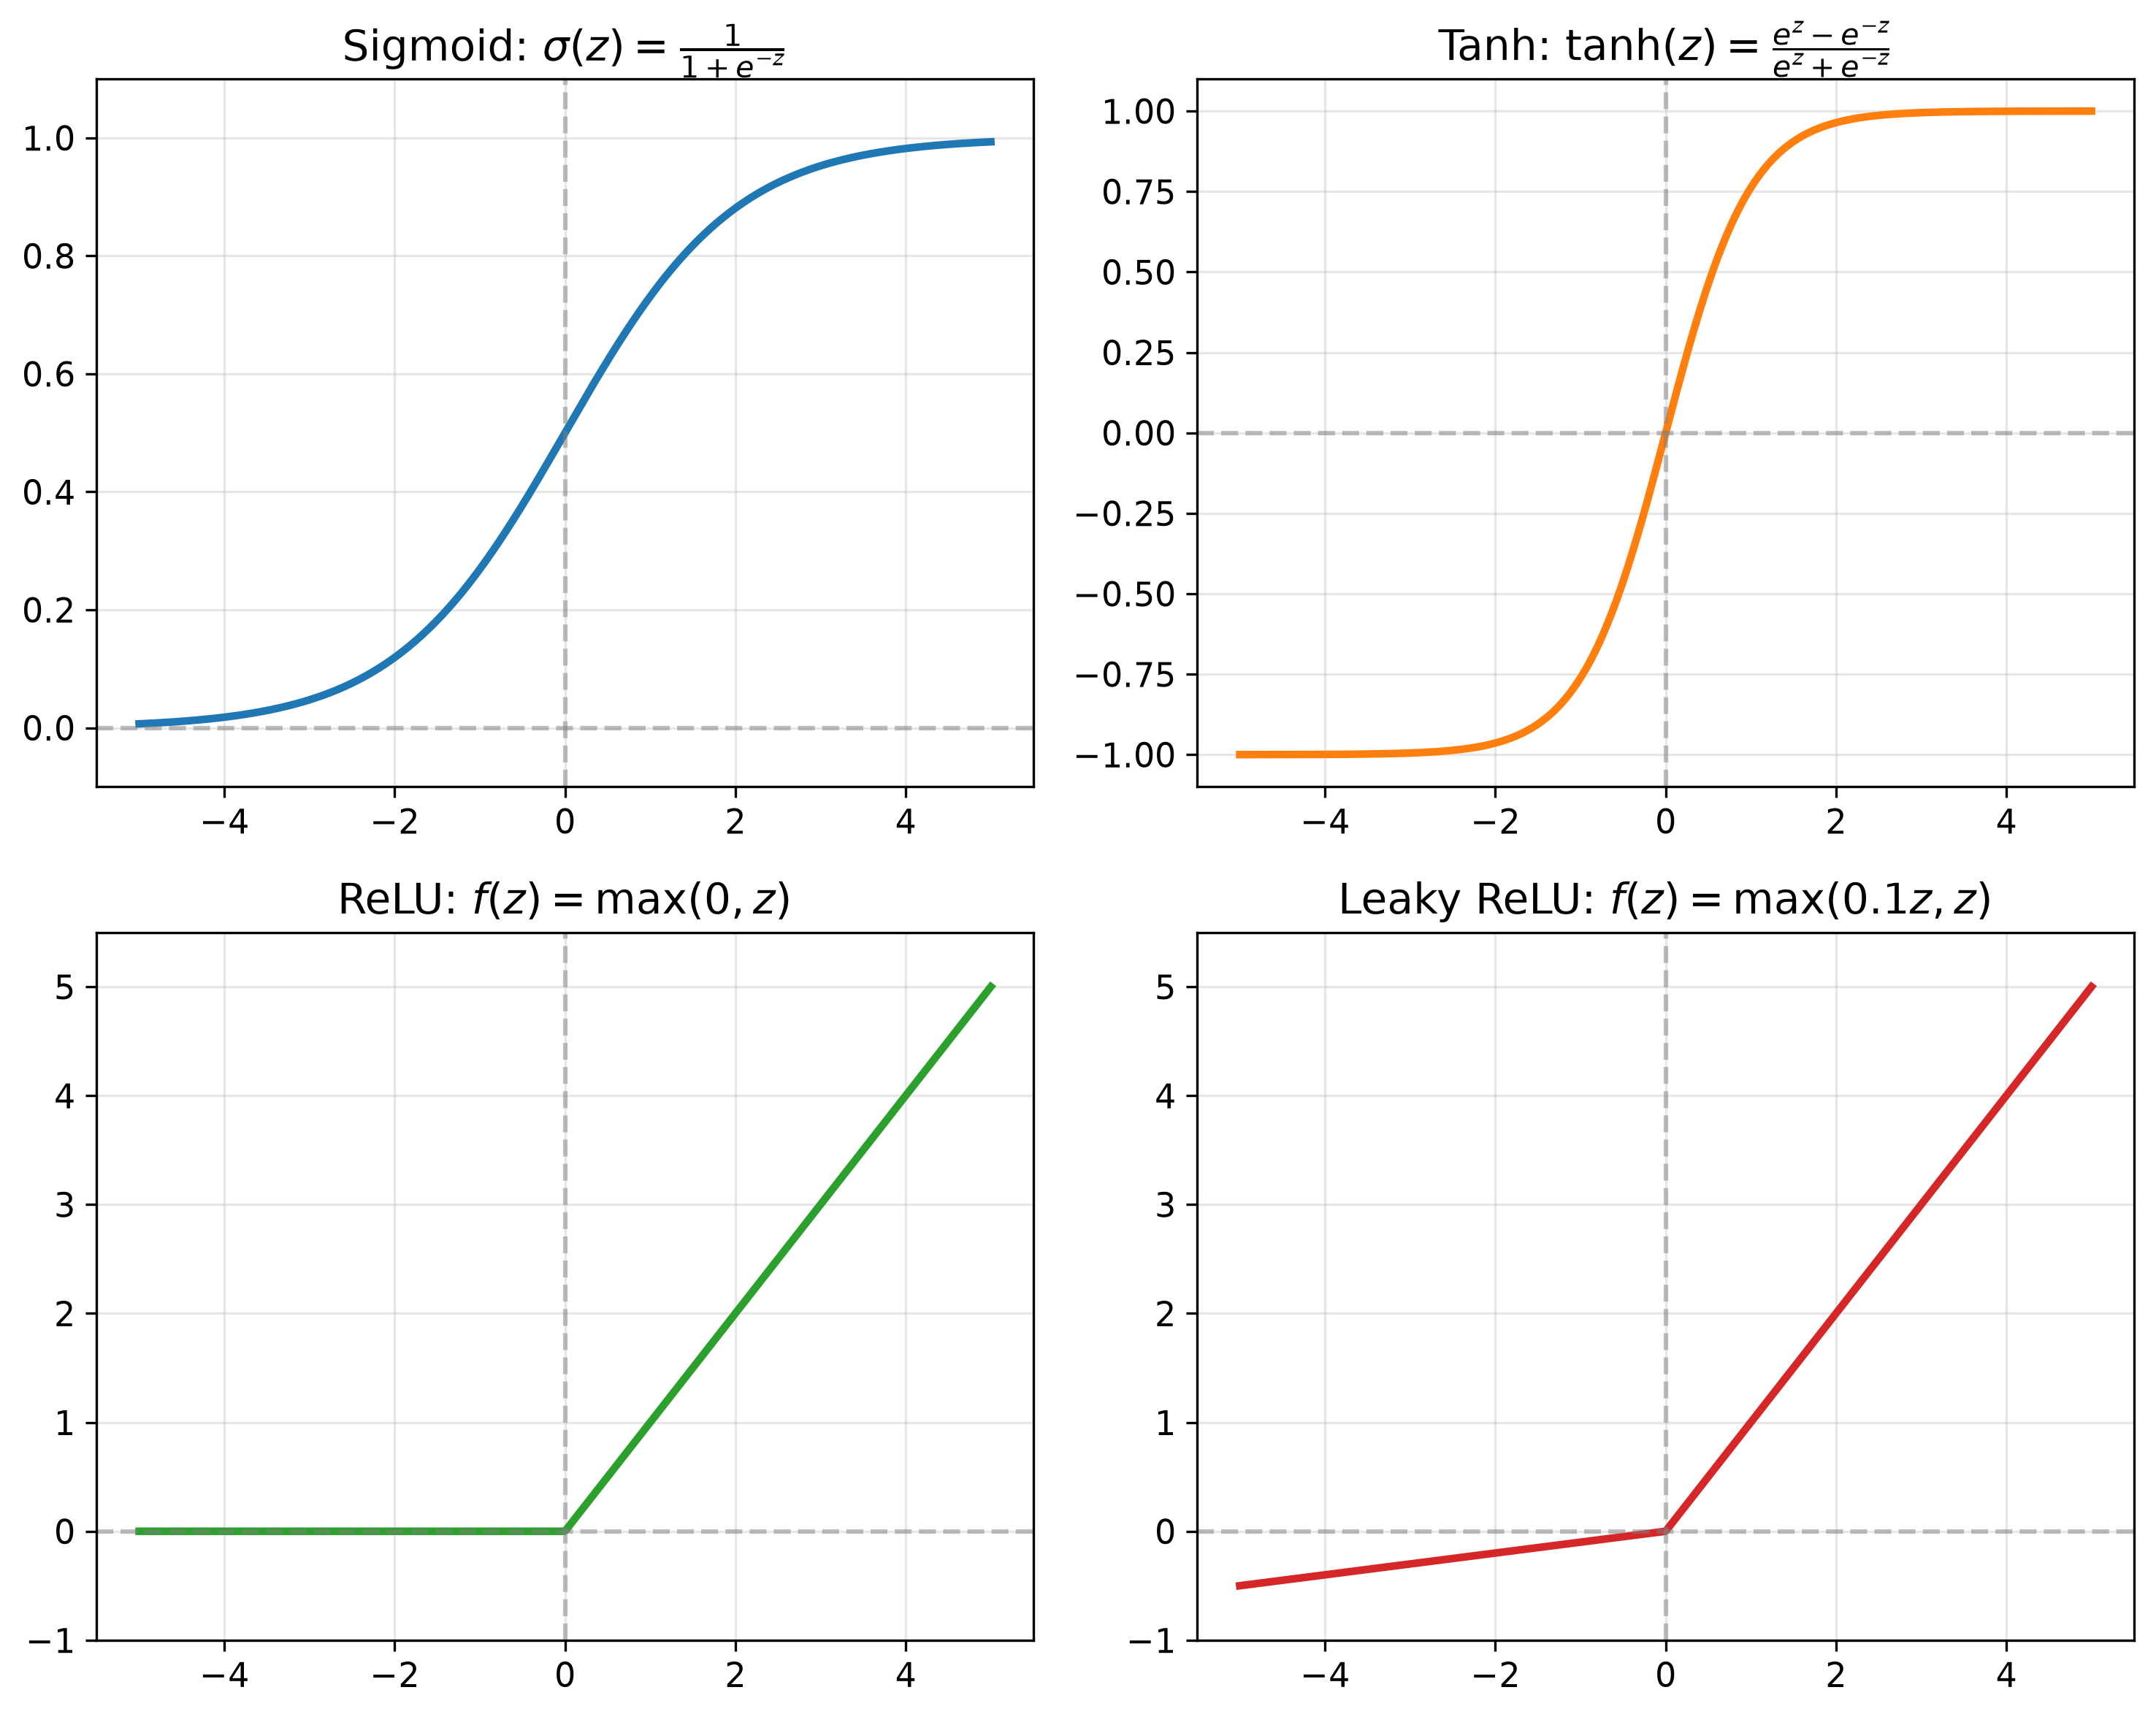
\includegraphics[width=0.75\linewidth,height=\textheight,keepaspectratio]{imagens/funcoes_ativacao.png}
\end{center}

\textbf{Falas do Apresentador:} ``Como vemos no gráfico comparativo das
quatro principais funções de ativação: - \textbf{Sigmoid}: Ideal para a
camada de saída em classificação binária, achatando valores para {[}0,
1{]}. - \textbf{Tanh}: Centrada em zero {[}-1, 1{]}, facilita a
convergência em camadas internas de redes recorrentes. - \textbf{ReLU}:
f(z) = max(0, z), o padrão absoluto para camadas ocultas em Deep
Learning moderno. - \textbf{Leaky ReLU}: Permite uma pequena inclinação
em valores negativos para evitar neurônios mortos.''

\begin{center}\rule{0.5\linewidth}{0.5pt}\end{center}

\subsection{A Função ReLU (Rectified Linear
Unit)}\label{a-funuxe7uxe3o-relu-rectified-linear-unit}

\[f(z) = \max(0, z)\]

\[f'(z) = \begin{cases} 0 & \text{se } z < 0 \\ 1 & \text{se } z > 0 \end{cases}\]

\begin{center}
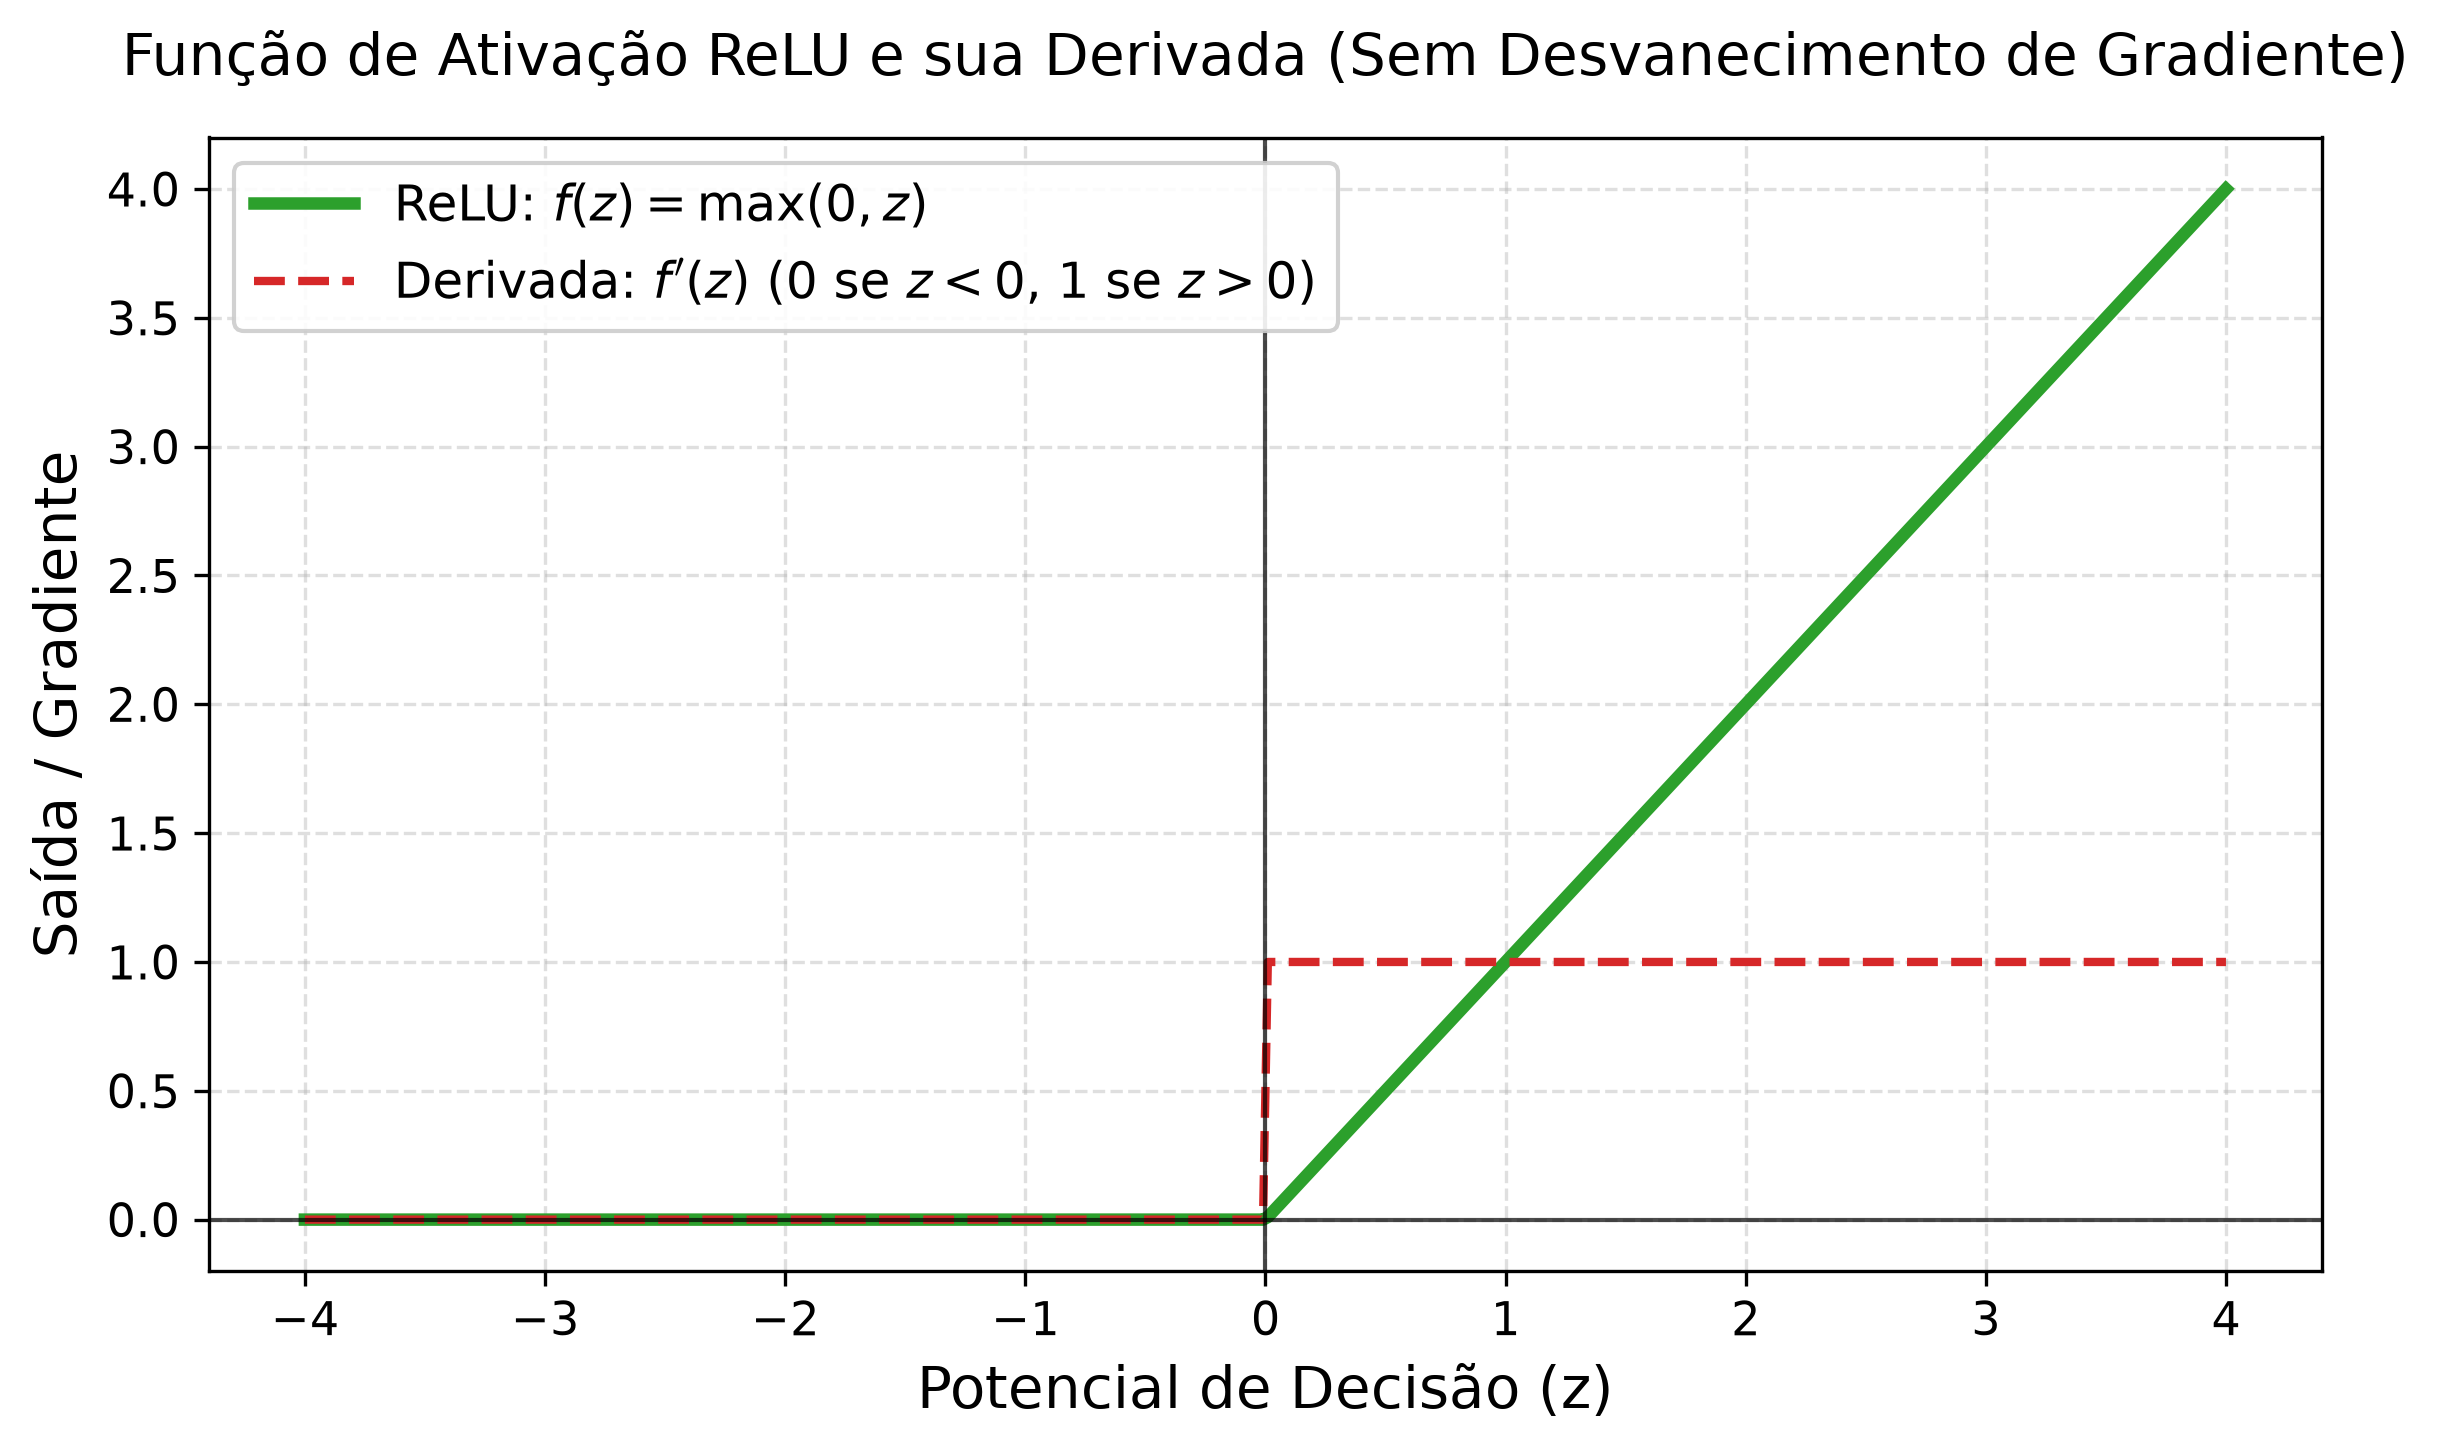
\includegraphics[width=0.9\linewidth,height=\textheight,keepaspectratio]{imagens/relu.png}
\end{center}

\textbf{Falas do Apresentador:} ``Esta é a ReLU, a função de ativação
mais utilizada no mundo do Deep Learning moderno. - \textbf{Definição
Matemática}: f(z) é igual a zero se z for menor ou igual a zero, e igual
a z se z for positivo. - \textbf{Derivada}: Observem a linha vermelha
tracejada no gráfico: para qualquer valor positivo z \textgreater{} 0, o
gradiente da ReLU é constante e exatamente igual a 1.0! - Essa
característica de derivada constante igual a 1.0 é fundamental para o
aprendizado em redes profundas.''

\begin{center}\rule{0.5\linewidth}{0.5pt}\end{center}

\subsection{Vantagens da Função
ReLU}\label{vantagens-da-funuxe7uxe3o-relu}

\begin{enumerate}
\def\labelenumi{\arabic{enumi}.}
\tightlist
\item
  \textbf{Simplicidade Computacional}
\item
  \textbf{Gradiente Constante (Combate ao Vanishing Gradient)}
\item
  \textbf{Esparsidade de Representação}
\end{enumerate}

\textbf{Falas do Apresentador:} ``Por que essa função tão simples
superou a Sigmoid e a Tanh nas camadas ocultas? 1. \textbf{Simplicidade
Computacional}: A ReLU exige apenas comparar se o valor é maior que zero
(if z \textgreater{} 0), economizando bilhões de operações exponenciais
em GPUs. 2. \textbf{Gradiente Constante}: Como a derivada é 1.0 para z
\textgreater{} 0, o sinal do erro flui sem atenuação durante o
backpropagation, combatendo o desvanecimento do gradiente. 3.
\textbf{Esparsidade}: Zera neurônios inativos (z \textless= 0), fazendo
com que apenas as características mais relevantes fiquem ativas.''

\begin{center}\rule{0.5\linewidth}{0.5pt}\end{center}

\subsection{A Variante Leaky ReLU}\label{a-variante-leaky-relu}

\[f(z) = \max(\alpha z, z) \quad (\text{onde } \alpha = 0.1)\]

\textbf{Falas do Apresentador:} ``Embora a ReLU seja fantástica, ela
possui uma limitação conhecida como `Neurônio Morto' (Dying ReLU). Se
durante o treinamento a entrada de um neurônio se tornar
consistentemente negativa, a saída será sempre zero e o gradiente também
será zero, impedindo a atualização dos pesos. A Leaky ReLU resolve isso
introduzindo uma inclinação suave (como 0.1 * z) para valores negativos.
Assim, mesmo neurônios inativos continuam recebendo uma fração de
gradiente para poderem voltar a aprender durante o treinamento.''

\begin{center}\rule{0.5\linewidth}{0.5pt}\end{center}

\subsection{O Desafio dos Problemas
Não-Lineares}\label{o-desafio-dos-problemas-nuxe3o-lineares}

\subsubsection{Problemas Lineares}\label{problemas-lineares}

\begin{itemize}
\tightlist
\item
  Dados separáveis por uma única reta ou plano.
\end{itemize}

\subsubsection{Problemas Não-Lineares
(XOR)}\label{problemas-nuxe3o-lineares-xor}

\begin{itemize}
\tightlist
\item
  Classes cruzadas em quadrantes. Nenhuma reta consegue separar sem
  erros.
\end{itemize}

\textbf{Falas do Apresentador:} ``No mundo real, quase nenhum problema
de imagem, texto ou negócios é linearmente separável. Se tentarmos
desenhar qualquer linha reta para separar dados no padrão XOR, nós
SEMPRE vamos errar metade das amostras.''

\begin{center}\rule{0.5\linewidth}{0.5pt}\end{center}

\subsection{Demonstração Gráfica: Curvando o
Espaço}\label{demonstrauxe7uxe3o-gruxe1fica-curvando-o-espauxe7o}

\begin{center}
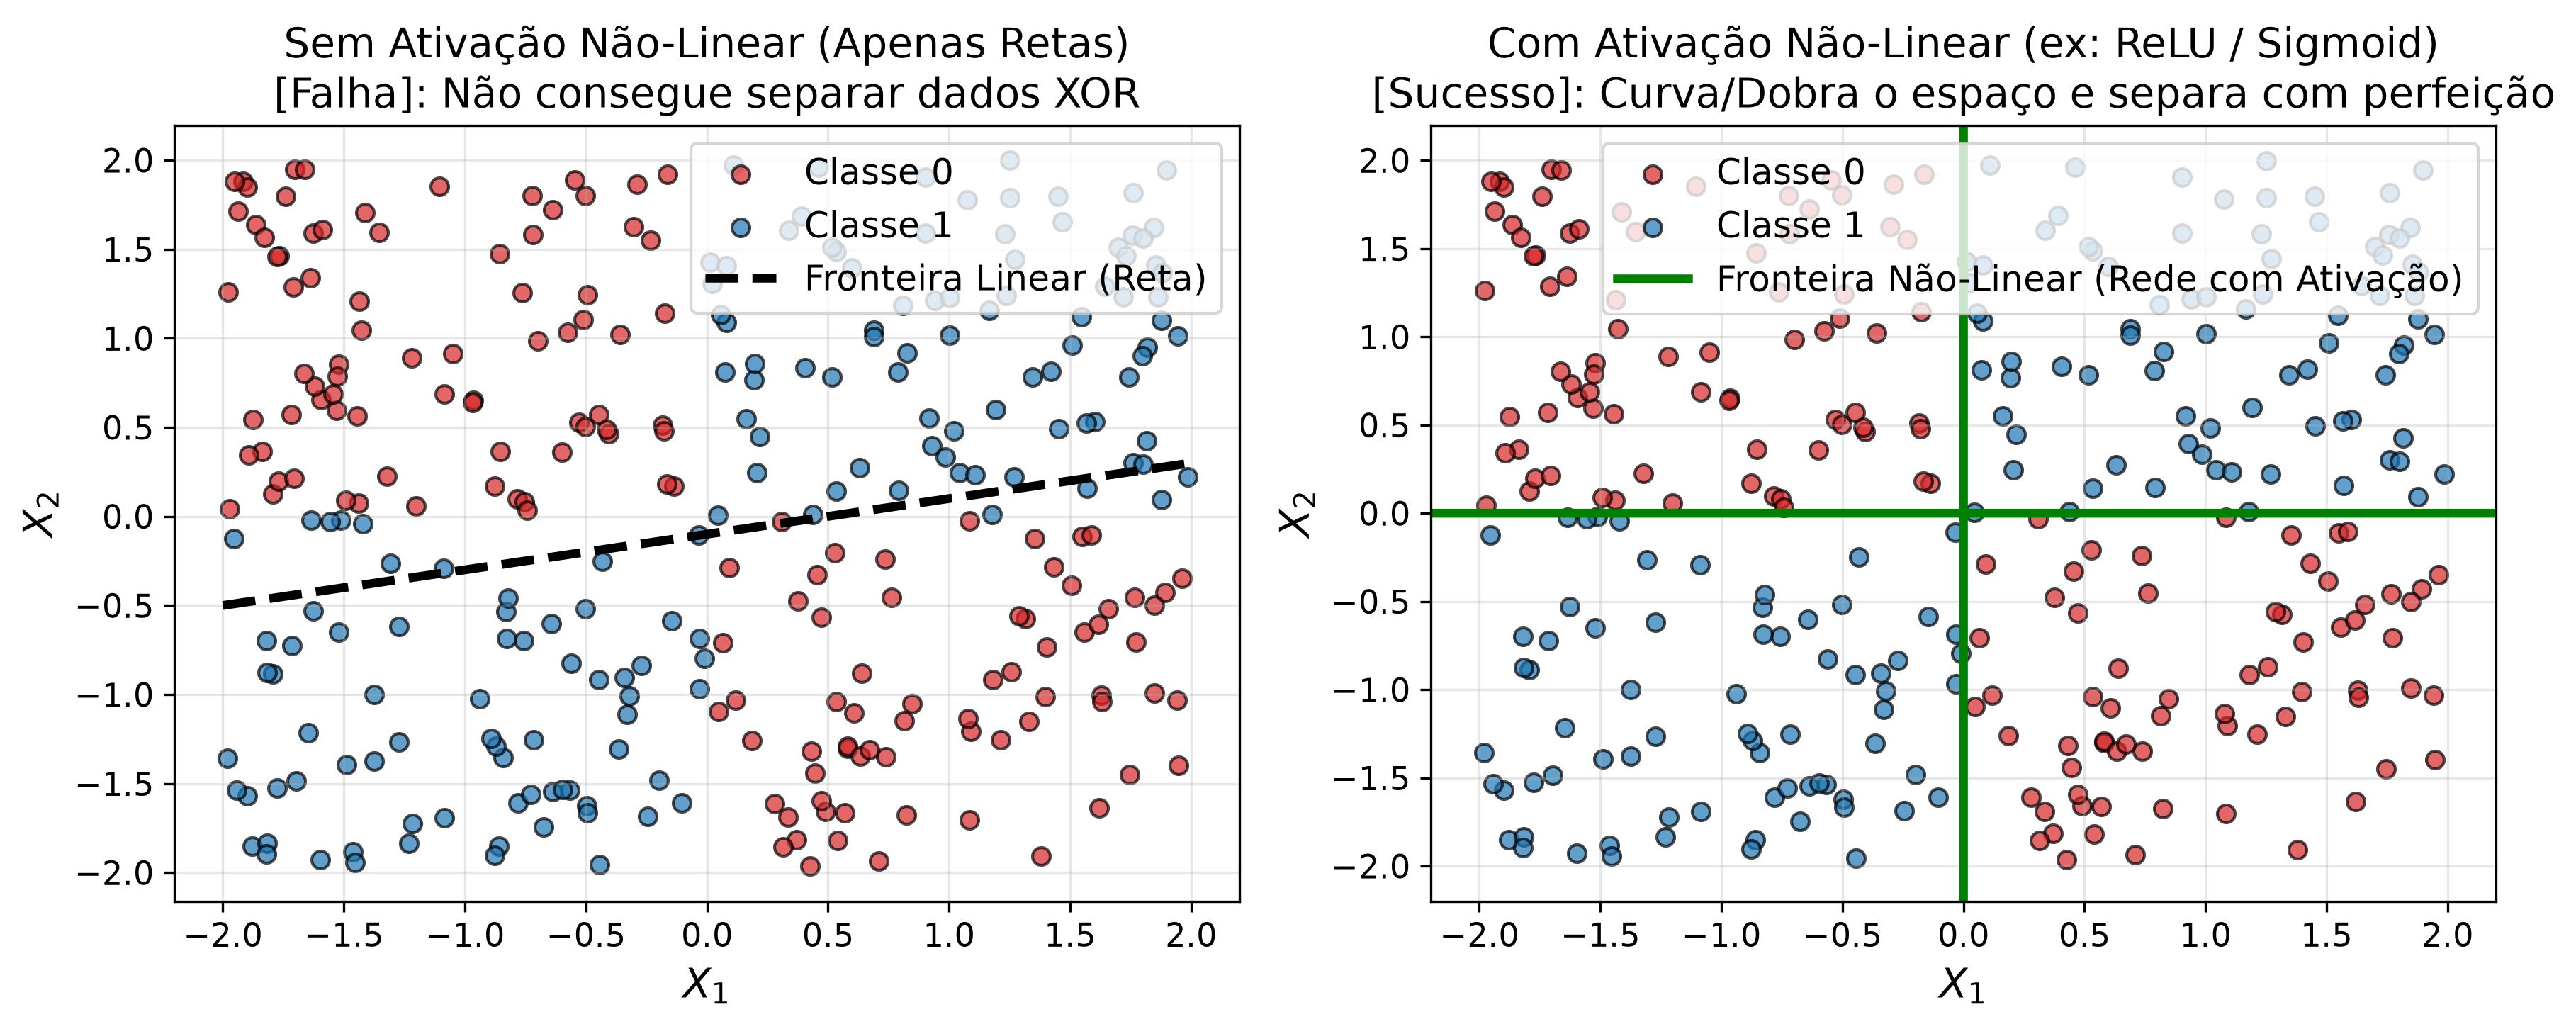
\includegraphics[width=0.75\linewidth,height=\textheight,keepaspectratio]{imagens/problema_nao_linear.png}
\end{center}

\textbf{Falas do Apresentador:} ``No gráfico da esquerda, um modelo
linear simples falha ao tentar separar os dados XOR com uma reta. No
gráfico da direita, ao adicionar uma camada oculta com funções de
ativação (como ReLU ou Sigmoid), a rede ganha a capacidade de criar
curvas de decisão perfeitas! É essa propriedade de curvar/distorcer o
espaço cartesiano que permite às redes neurais profundas resolverem
tarefas complexas de Visão Computacional e NLP.''

\begin{center}\rule{0.5\linewidth}{0.5pt}\end{center}

\subsection{Indo Além: Redes Multicamadas
(MLP)}\label{indo-aluxe9m-redes-multicamadas-mlp}

\begin{center}
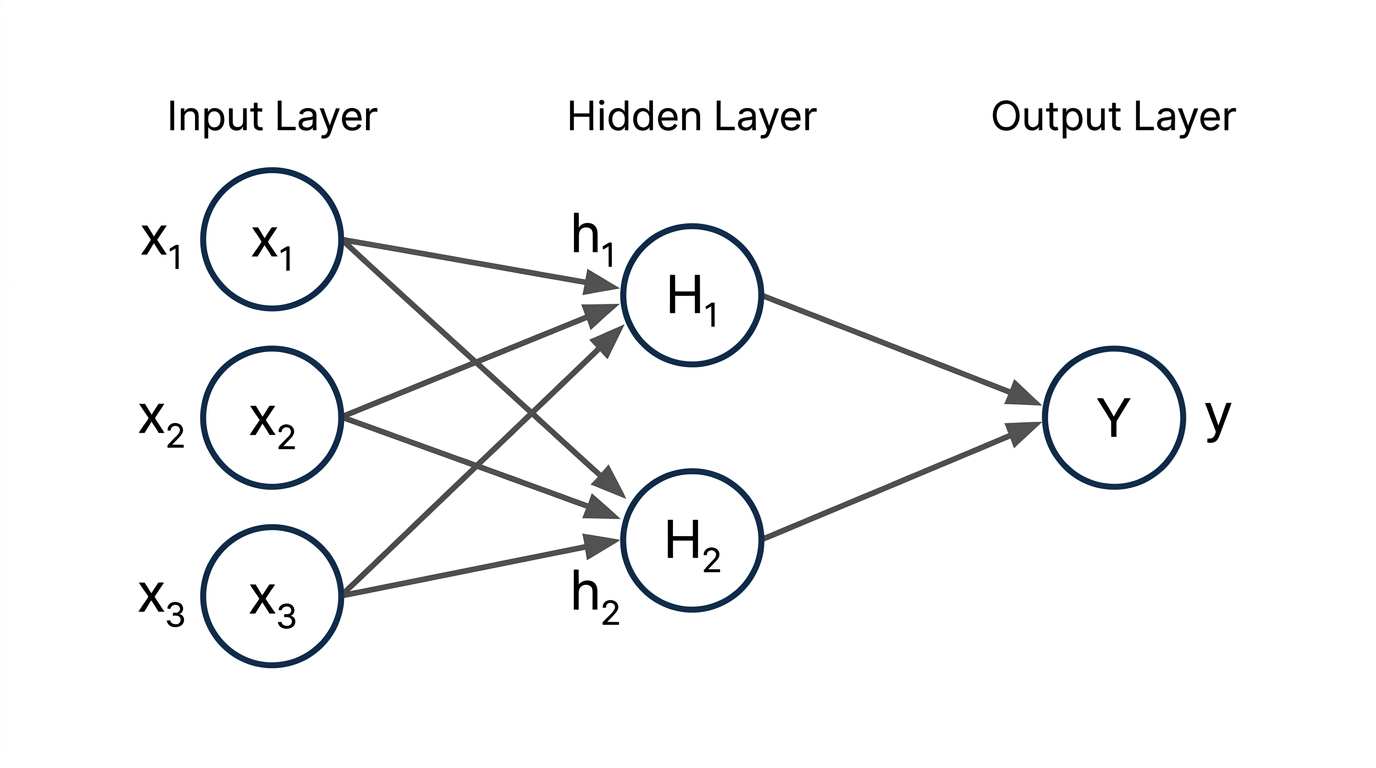
\includegraphics[width=0.65\linewidth,height=\textheight,keepaspectratio]{imagens/mlp_estrutura.jpg}
\end{center}

\textbf{Falas do Apresentador:} ``Para combinar múltiplos neurônios e
resolver esses problemas complexos, nós os organizamos em camadas,
formando uma MLP (Multi-Layer Perceptron). Como vemos no diagrama: 1.
\textbf{Camada de Entrada}: Recebe dados brutos (x1, x2, x3). 2.
\textbf{Camada Oculta}: Neurônios intermediários (h1, h2) que extraem
representações não-lineares. 3. \textbf{Camada de Saída}: O neurônio
final (y) gera a resposta combinada.''

\begin{center}\rule{0.5\linewidth}{0.5pt}\end{center}

\subsection{Matemática da MLP: Camada
Oculta}\label{matemuxe1tica-da-mlp-camada-oculta}

\[h_1 = \sigma(w_{11} x_1 + w_{21} x_2 + w_{31} x_3 + b_{h1})\]

\[h_2 = \sigma(w_{12} x_1 + w_{22} x_2 + w_{32} x_3 + b_{h2})\]

\textbf{Falas do Apresentador:} ``Cada neurônio da camada oculta (h1 e
h2) é um Perceptron completo processando as mesmas entradas de forma
independente. - h1 multiplica as entradas x1, x2, x3 pelos pesos da
primeira linha, adiciona o viés b\_h1 e aplica a Sigmoid. - h2 faz o
mesmo cálculo usando seu próprio conjunto de pesos e viés b\_h2. Cada
neurônio aprende a detectar um aspecto ou característica diferente dos
dados.''

\begin{center}\rule{0.5\linewidth}{0.5pt}\end{center}

\subsection{Matemática da MLP: Camada de
Saída}\label{matemuxe1tica-da-mlp-camada-de-sauxedda}

\[\hat{y} = \sigma(v_1 h_1 + v_2 h_2 + b_o)\]

\textbf{Falas do Apresentador:} ``Na camada de saída, o neurônio final
trata os valores processados por h1 e h2 como suas novas entradas. Ele
aplica os pesos v1 e v2 da segunda camada, adiciona o viés de saída b\_o
e passa pela Sigmoid para produzir a probabilidade final y-chapéu.''

\begin{center}\rule{0.5\linewidth}{0.5pt}\end{center}

\subsection{Dinâmica com Planilha: Ajustando o
Neurônio}\label{dinuxe2mica-com-planilha-ajustando-o-neuruxf4nio}

\begin{itemize}
\tightlist
\item
  \textbf{Arquivo}: \texttt{simulacao\_perceptron.xlsx}
\item
  \textbf{Objetivo}: Mudar \(W_1\), \(W_2\) e \(Bias\) para classificar
  os 20 atletas e zerar a Loss.
\end{itemize}

\textbf{Falas do Apresentador:} ``Preparamos uma planilha interativa
chamada simulacao\_perceptron.xlsx. Nela, constam os dados de 20
atletas. Vocês devem alterar manualmente as variáveis de W1, W2 e Bias
na planilha para ver a reta divisória se ajustar e a perda despencar.''

\begin{center}\rule{0.5\linewidth}{0.5pt}\end{center}

\subsection{Transição para o
PyTorch}\label{transiuxe7uxe3o-para-o-pytorch}

\subsubsection{1. Tensores}\label{tensores}

\begin{itemize}
\tightlist
\item
  Arrays multidimensionais em GPU.
\end{itemize}

\subsubsection{2. Autograd}\label{autograd}

\begin{itemize}
\tightlist
\item
  Diferenciação automática de gradientes.
\end{itemize}

\subsubsection{3. Otimizadores}\label{otimizadores}

\begin{itemize}
\tightlist
\item
  Ajuste automático dos pesos (SGD, Adam).
\end{itemize}

\begin{quote}
\textbf{Próximo Passo}: Abrir o Jupyter Notebook
\texttt{aula\_01\_introducao\_deep\_learning.ipynb}!
\end{quote}

\textbf{Falas do Apresentador:} ``O PyTorch substitui nosso ajuste
manual por três pilares: Tensores, Autograd e Otimizadores. Vamos agora
abrir o nosso Jupyter Notebook!''




\end{document}
